% !TEX root = main.tex

\subsection{Learn From Rule}

\begin{figure}[!]
    \centering
    % \vspace{-0.2em}
    \begin{subfigure}[]{0.24\textwidth}
        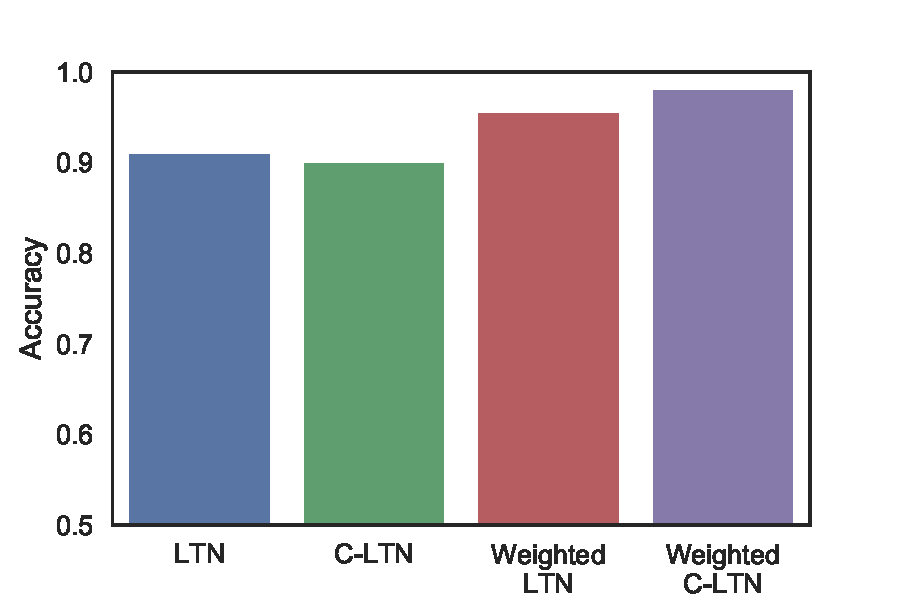
\includegraphics[width=\textwidth]{img/bar3.pdf}
        \caption{Best Accuracy on Group1}
        \label{fig:learning-best-accuracy-1}
        %\vspace{-0.3em}
    \end{subfigure}~~~~
    \begin{subfigure}[]{0.24\textwidth}
        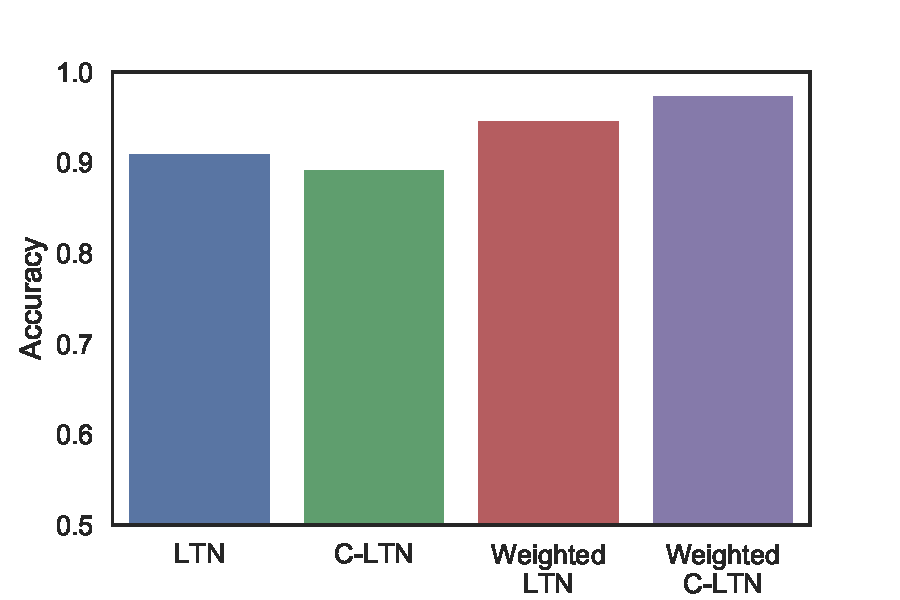
\includegraphics[width=\textwidth]{img/bar4.pdf}
        \caption{Best Accuracy on Group2}
        \label{fig:learning-best-accuracy-2}
        %\vspace{-0.8em}
    \end{subfigure}

    \begin{subfigure}[]{0.24\textwidth}
        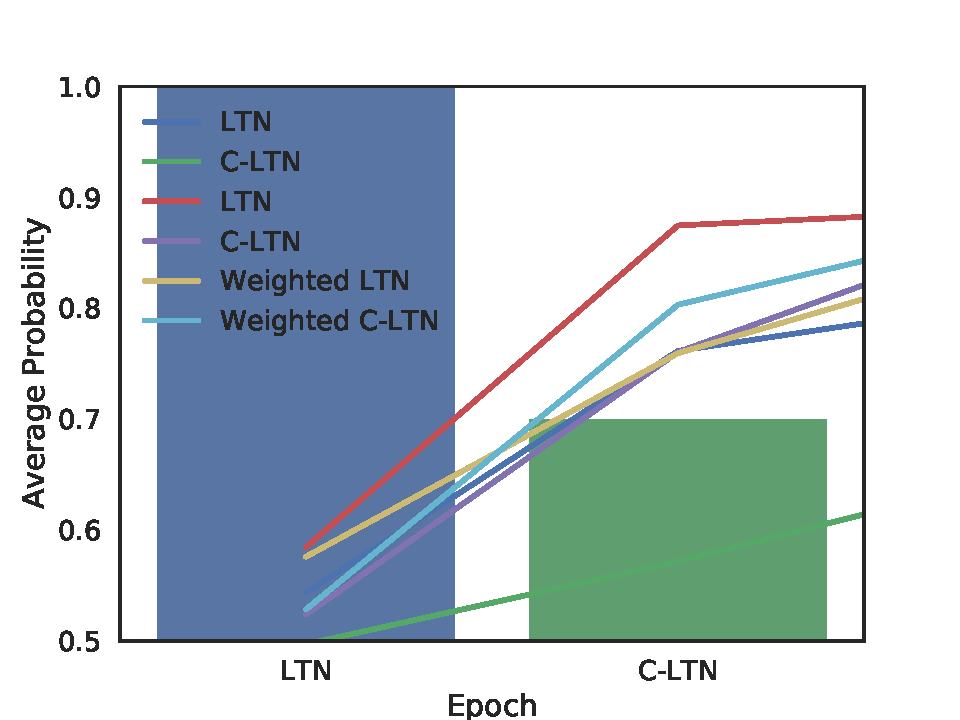
\includegraphics[width=\textwidth]{img/curve2.pdf}
        \caption{Probability w.r.t. Epoch}
        \label{fig:learning-prob-epoch}
        %\vspace{-0.3em}
    \end{subfigure}
    \caption{Learning from Observed Facts \& Rules.}
    \label{fig:learning}
    % \vspace{-1.2em}
\end{figure}

Firgure \ref{fig:learning} shows the result of two models on datasets. Like the result in last subsection, this figure containts three subfigures, including probability changes and best accuracy on two groups.

Some interesting phenomenon can be concluded from the results.

First, by comparing results on weighted and unweighted dataset, we can see that training on weighted dataset gets a better performance.
As we said before, this is because the weighted method treat each proposal as one clause, which could avoid the unbalanced training.

Second, C-LTN on weighted datasets shows the best performance. That's because CNN has better fitting ability and more stable in training.

\begin{table}[]
\centering
\begin{tabular}{c|c|c|cccccccc}
\toprule
\multirow{2}{*}{} & \multirow{2}{*}{S} & \multirow{2}{*}{C} & \multicolumn{8}{l}{F}                                 \\ \cmidrule{4-11}
                  &                    &                    & a    & b    & c    & d    & e    & f    & g    & h    \\ \midrule
a                 & 1.00               & 1.00               & 1.00 & 1.00 & 0.00 & 0.00 & 1.00 & 1.00 & 1.00 & 0.00 \\
b                 & 0.00               & 0.00               & 1.00 & 0.05 & 1.00 & 0.00 & 0.00 & 0.00 & 0.00 & 0.00 \\
c                 & 0.00               & 0.00               & 0.00 & 1.00 & 0.93 & 1.00 & 0.00 & 0.00 & 0.00 & 0.00 \\
d                 & 0.00               & 0.00               & 0.00 & 0.00 & 1.00 & 0.00 & 0.00 & 0.00 & 0.00 & 0.00 \\
e                 & 1.00               & 1.00               & 1.00 & 0.00 & 0.00 & 0.00 & 0.00 & 1.00 & 0.00 & 0.00 \\
f                 & 1.00               & 0.00               & 1.00 & 0.00 & 0.00 & 0.00 & 1.00 & 0.01 & 0.00 & 0.00 \\
g                 & 0.49               & 0.00               & 1.00 & 0.00 & 0.00 & 0.00 & 0.00 & 0.00 & 0.10 & 1.00 \\
h                 & 0.00               & 0.00               & 0.00 & 0.00 & 0.00 & 0.00 & 0.00 & 0.00 & 1.00 & 0.00 \\ \bottomrule
\end{tabular}
\caption{Fitting and Learning on Group1}
\label{table:learning-group-1}
\end{table}

\begin{table}[]
\centering
\begin{tabular}{c|c|c|cccccc}
\toprule
\multirow{2}{*}{} & \multirow{2}{*}{S} & \multirow{2}{*}{C} & \multicolumn{6}{l}{F}                   \\ \cmidrule{4-9}
                  &                    &                    & i    & j    & k    & l    & m    & n    \\ \midrule
i                 & 1.00               & 0.84               & 0.13 & 1.00 & 0.00 & 0.00 & 1.00 & 0.00 \\
j                 & 0.00               & 0.25               & 1.00 & 0.00 & 0.00 & 0.00 & 0.00 & 0.00 \\
k                 & 0.00               & 0.76               & 0.00 & 0.00 & 0.13 & 1.00 & 0.00 & 0.03 \\
l                 & 0.00               & 0.08               & 0.00 & 0.00 & 1.00 & 0.05 & 0.00 & 0.00 \\
m                 & 0.00               & 0.54               & 1.00 & 0.00 & 0.00 & 0.00 & 0.32 & 1.00 \\
n                 & 1.00               & 0.04               & 0.00 & 0.00 & 0.03 & 0.00 & 1.00 & 0.05 \\ \bottomrule
\end{tabular}
\caption{Fitting and Learning on Group2}
\label{table:learning-group-2}
\end{table}

\begin{table}[]
\centering
\begin{tabular}{lll}
\toprule
Propositional           & Group1   & Group2   \\ \midrule
$\forall \neg F(x, x)$                & 0.625    & 0.5      \\
$\forall x y F(x,y)\rightarrow F(y,x) $      & 0.984375 & 0.916667 \\
$\forall x \exists y F(x,y) $                 & 1        & 1        \\
$\forall x y S(x) F(x,y)\rightarrow S(y) $ & 0.9375   & 0.916667 \\
$\forall x S(x)\rightarrow C(x) $            & 0.75     & 0.666667 \\ \bottomrule
\end{tabular}
\caption{Learned Rules}
\label{table:learning-learned-rules}
\end{table}
